\setcounter{subsection}{0}
\section{ANÁLISIS DEL PROBLEMA}

El SRS (IEEE 830 e ISO/IEC/IEEE 29148) especificó 60 requerimientos: 45 funcionales (RF), 4 de desempeño (RD) y 11 no funcionales (RNF), agrupados en nueve módulos funcionales y en atributos de calidad. Esta sección resume los más importantes; el detalle está en el SRS (anexos).

\subsection{Requerimientos}

\textbf{Usuarios.} Se identificaron tres clases: el investigador o analista de datos (ejecuta el \textit{pipeline} con distintas configuraciones), el desarrollador del equipo y el planificador o analista de movilidad no técnico, que usa solo la interfaz web y no necesita saber Python ni SUMO. Este último fue el usuario de referencia para el diseño de la interfaz.

\textbf{Requerimientos funcionales.} La tabla~\ref{tab:requerimientos} resume los módulos, con los requerimientos más relevantes de cada uno.

\begin{table}[ht]
\renewcommand{\arraystretch}{1.15}
\centering
\small
\begin{tabular}{|p{1.6cm}|p{3.4cm}|p{9cm}|}
\hline
\textbf{Módulo} & \textbf{Nombre} & \textbf{Capacidades principales} \\ \hline
F1 & Ingestión y validación & Leer la encuesta, validar columnas y conteo de filas descartadas, limpieza y expansión muestral con \texttt{fexp\_vj}. \\ \hline
F2 & Matrices O/D & Matrices por modo y periodo; en la implementación, viajes por TAZ ordenados por hora de salida. \\ \hline
F3 & Red y TAZ & Red 3D de Usaquén con \texttt{netconvert} y zonas TAZ. \\ \hline
F4 & Archivos de simulación & Tipos de vehículo por modo, \texttt{trips.xml}, rutas con \texttt{duarouter}. \\ \hline
F5 & Variación paramétrica & Presets de transferencia modal, conteos por modo, semilla, estilos de conducción, cierres viales y simulaciones precalculadas. \\ \hline
F6 & Módulo web & Mapa animado por modo, panel de parametrización, avance real y cancelación de corridas. \\ \hline
F7 & Validación y reportes & GEH contra aforos HMD, \textit{log} estructurado, \textit{checkpoints}. \\ \hline
F8 & Intersecciones & Ficha de semáforos con volúmenes por acceso, edición de programas, Webster, recorte de zonas, priorización de cruces sin semáforo. \\ \hline
F9 & Simulador 3D & Comparación sin/con semáforo propuesto, actor en tercera persona, HUD, TTC/DRAC/PET, modo manual, minimapa. \\ \hline
\end{tabular}
\caption{Módulos funcionales del SRS.}
\label{tab:requerimientos}
\end{table}

\textbf{Requerimientos de desempeño.} RD-001: el \textit{pipeline} debe completarse en 4 horas como máximo en una máquina de 8~GB de RAM y 4 núcleos. RD-003: preparar una comparación 3D debe tardar a lo sumo 60~s. RD-004: el visor debe renderizar las dos escenas 3D a 30 cuadros por segundo o más con GPU integrada.

\textbf{Requerimientos no funcionales.} Se especificaron confiabilidad, disponibilidad, seguridad, mantenibilidad, portabilidad (Linux y Windows), reproducibilidad (misma entrada, misma salida), observabilidad y usabilidad. Dos de ellos condicionaron el diseño: la reproducibilidad (semilla explícita, orden determinista de viajes, huella SHA-256 de los insumos) y la usabilidad para un usuario no técnico (valores por defecto coherentes con la encuesta, avance visible, mensajes en español).

\subsection{Restricciones}

\begin{itemize}[noitemsep]
    \item \textbf{Alcance geográfico:} la localidad de Usaquén; el diseño debe permitir extenderlo, pero hoy extenderlo exige preparar los insumos de cada escenario.
    \item \textbf{Uso:} el sistema es monousuario; la API ejecuta una corrida pesada a la vez y como máximo dos comparaciones 3D simultáneas.
    \item \textbf{Software:} Python 3.11 o superior (servicio) y JavaScript con React (visor); solo bibliotecas de código abierto o de uso académico gratuito; la red y las rutas se generan con \texttt{netconvert} y \texttt{duarouter}, sin reimplementarlos; sin motor de base de datos (el almacenamiento es por archivos).
    \item \textbf{Hardware:} 8~GB de RAM, 4 núcleos y 10~GB libres como mínimo; el simulador 3D requiere un navegador con WebGL~2.
    \item \textbf{Datos:} los microdatos crudos de la encuesta no se versionan; el repositorio solo contiene el TSV de viajes internos de Usaquén ya filtrado. Los programas semafóricos son los que genera \texttt{netconvert} desde OpenStreetMap (82~s de verde, 3~s de amarillo y 5~s de todo rojo), no los programas reales de la SDM.
    \item \textbf{Idioma y estilo:} código, comentarios, identificadores y documentación en español; estilo PEP~8.
    \item \textbf{Seguridad:} no hay autenticación ni cifrado; el sistema es una herramienta local de investigación.
\end{itemize}

También se aceptaron límites del dato: la simulación cubre la ventana de 7:00 a 10:00; el transporte público se representa como caminata (no hay buses, paradas ni GTFS); y las brechas de cobertura muestral y de atributos de OSM identificadas en la Fase 1 (sección~\ref{sec:fase1}).

\subsection{Especificación Funcional}

La especificación funcional se organizó en 12 casos de uso agrupados por actor. El investigador ejecuta el \textit{pipeline} (CU-01 a CU-06: ingestión, matrices, red y TAZ, archivos de simulación, escenarios y validación). El planificador usa el módulo web para visualizar resultados y configurar simulaciones (CU-07 y CU-08), analizar intersecciones (CU-09 a CU-11) y comparar un cruce en 3D (CU-12).

La figura~\ref{fig:contexto} muestra el contexto del sistema (nivel 1 del modelo C4): dos tipos de usuarios, el sistema y las fuentes y herramientas externas con las que se relaciona.

\begin{figure}[H]
\centering
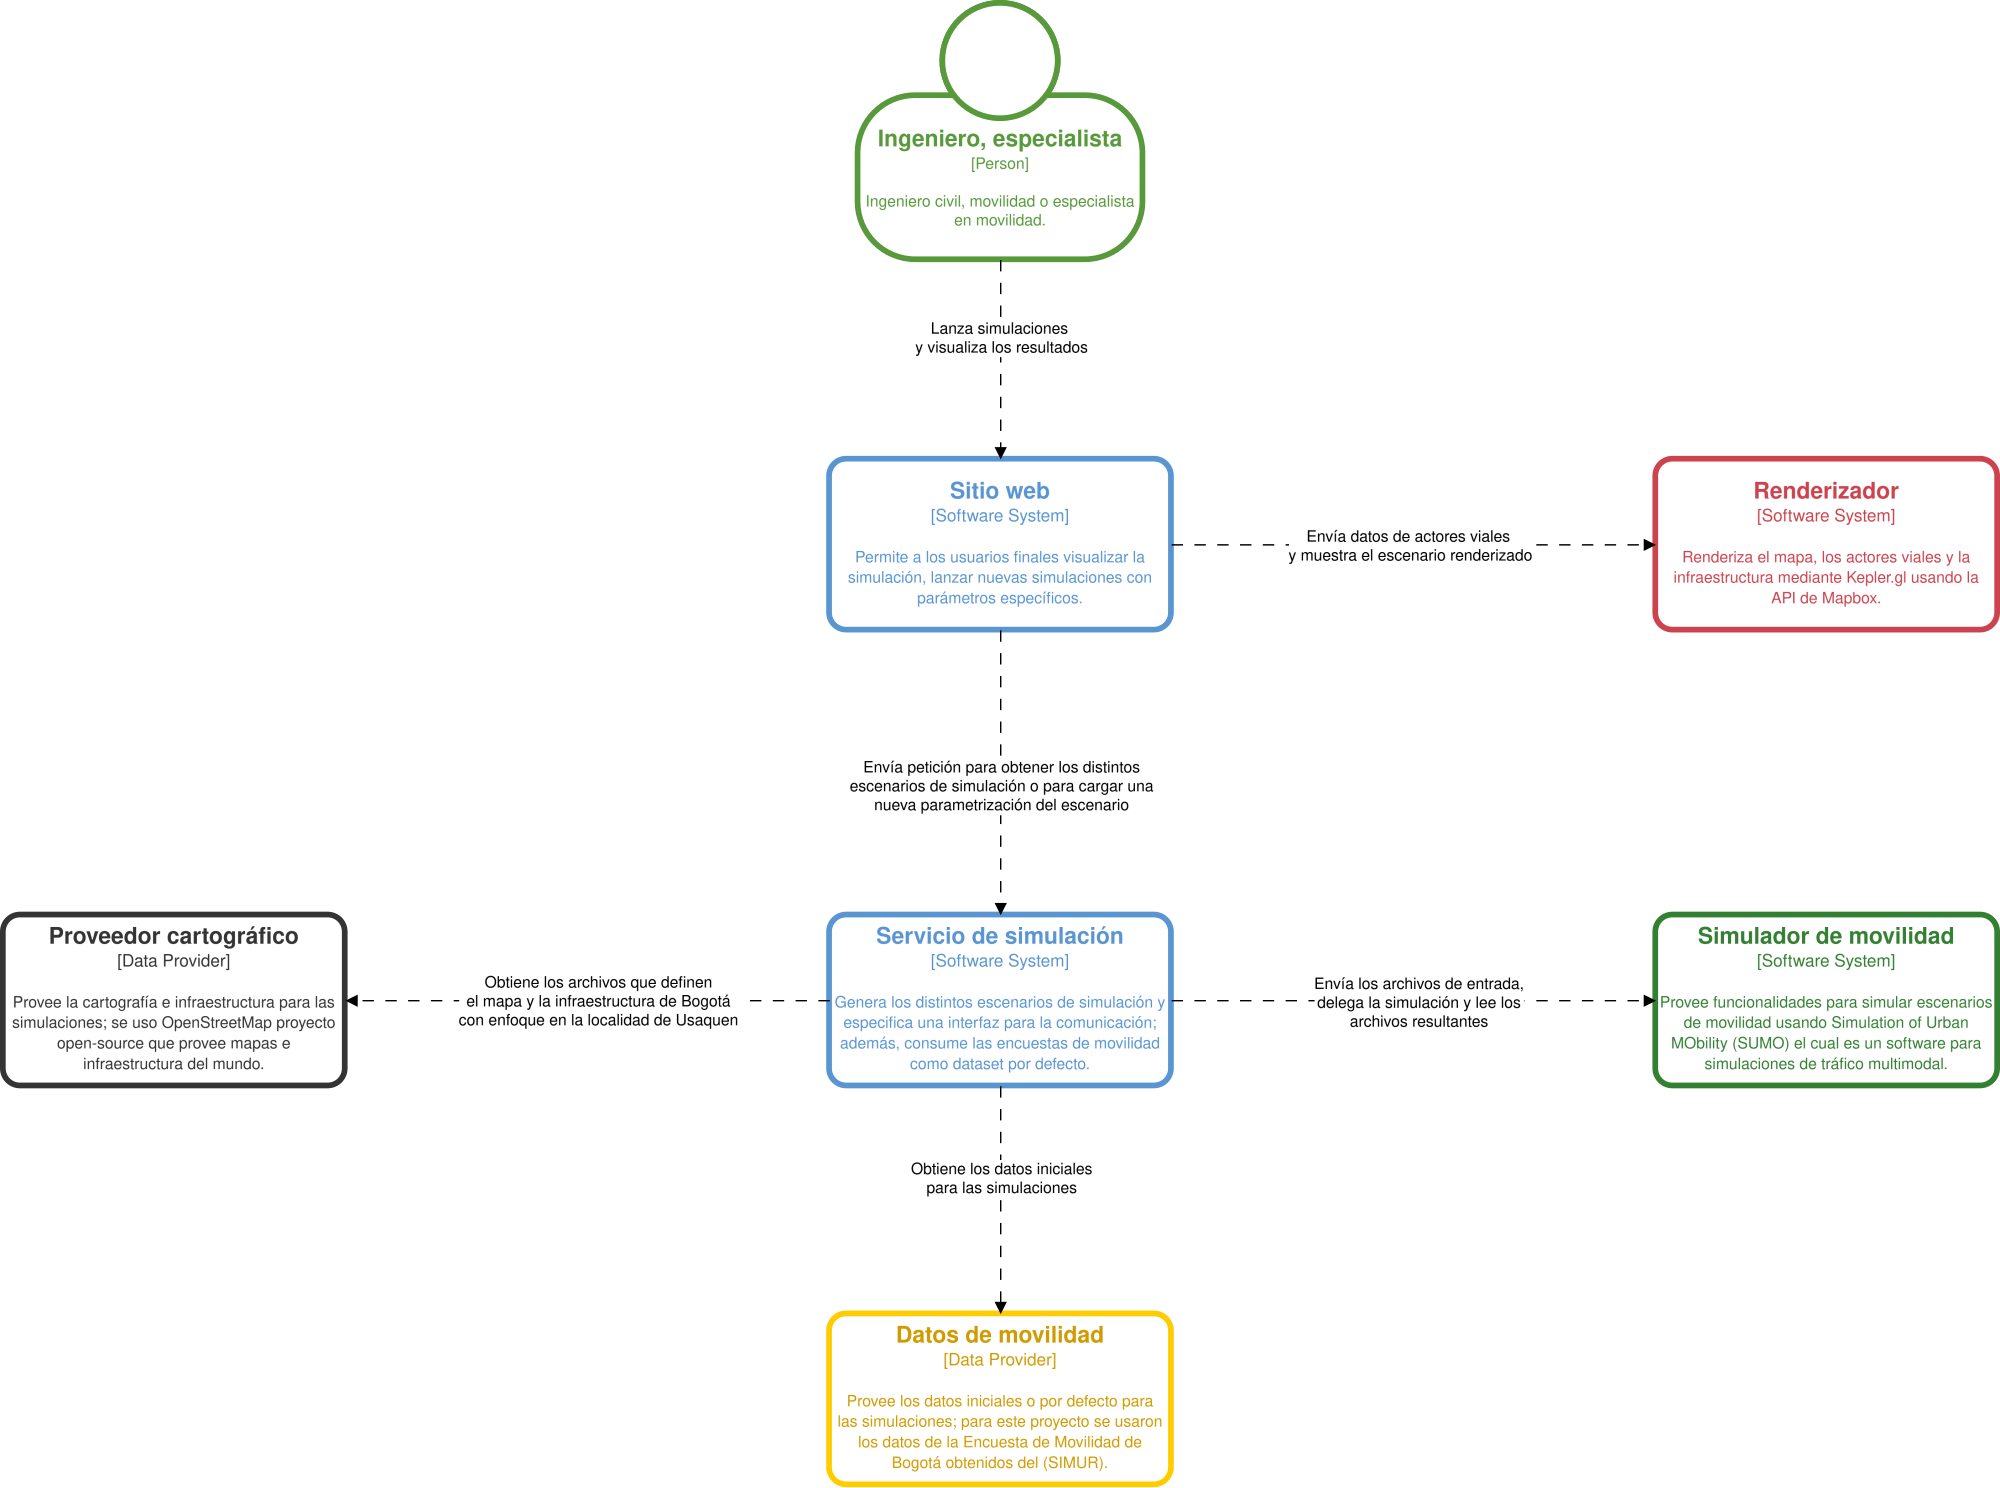
\includegraphics[width=0.95\textwidth]{c4-contexto.png}
\caption{Diagrama de contexto del sistema (modelo C4, nivel 1).}
\label{fig:contexto}
\end{figure}

\textbf{Flujos principales.}
\begin{enumerate}[noitemsep]
    \item \textit{Simulación parametrizada.} El usuario elige un preset de demanda, ajusta conteos, escala, semilla o estilo y lanza la corrida. El sistema genera los viajes, calcula las rutas, simula, exporta los resultados y el visor los anima. Mientras tanto muestra el avance real y permite cancelar.
    \item \textit{Simulación precalculada.} Los cuatro presets con sus conteos por defecto se simularon una vez y se versionaron; al abrir el visor se carga la simulación de la encuesta sin esperar.
    \item \textit{Análisis de intersecciones.} El usuario consulta un semáforo (accesos, volúmenes, fases), edita su programa o calcula uno con Webster, y compara programas. Además ve la priorización de cruces sin semáforo.
    \item \textit{Comparación 3D.} Para un cruce candidato, el sistema recorta la zona, crea la variante con semáforo, genera la demanda de la zona, y simula ambos escenarios en paralelo; el usuario sigue en tercera persona a un vehículo o peatón y observa velocidad, acción, decisiones posibles e índice de riesgo.
\end{enumerate}
